\section{Composi\c{c}\~ao de uma CDN} \label{sec:composicao}
\subsection{Tipos de servidores}
\begin{itemize}
	\item Servidor de origem
	\item Servidor de ponta
\end{itemize}
\begin{figure}[h]
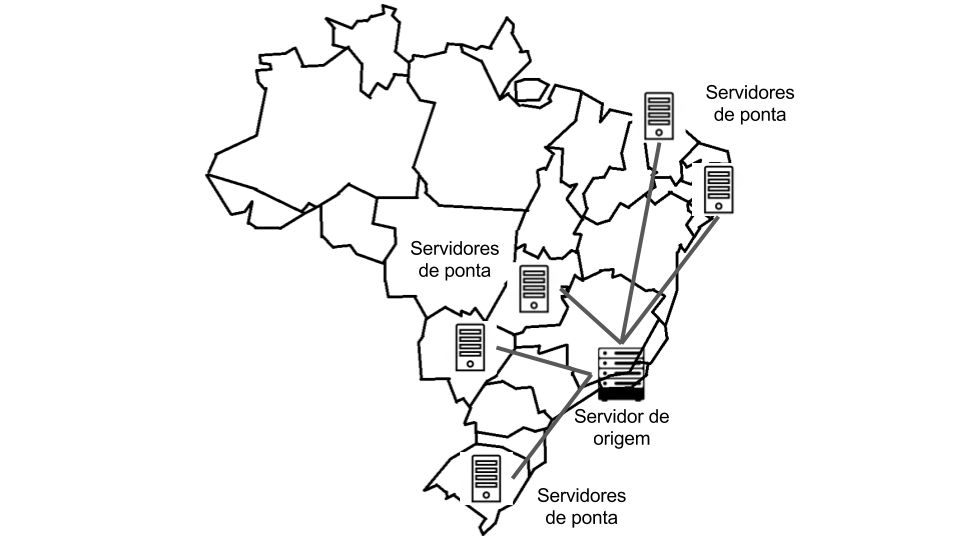
\includegraphics[width=10cm]{Figuras/tipos_servidores.png} 
\label{figura:tipos_servidores} 
\end{figure}

\subsection{Protocolos de intera\c{c}\~oes}

\begin{figure}[h]
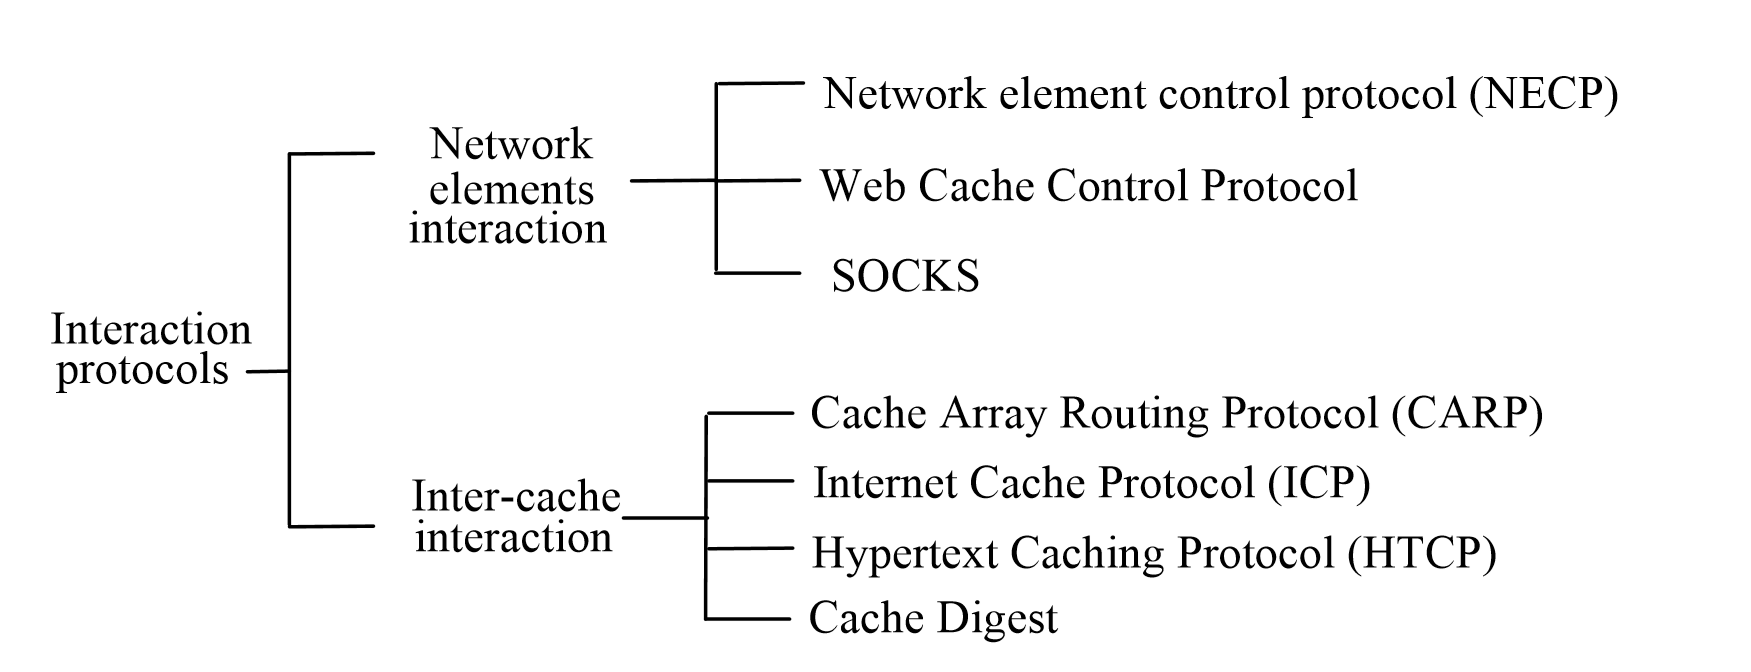
\includegraphics[width=10cm]{Figuras/tipos_relacionamentos.png} 
\label{figura:tipos_relacionamentos}
\end{figure}


\subsubsection{Intera\c{c}\~oes dos elementos da rede}
\begin{figure}[h]
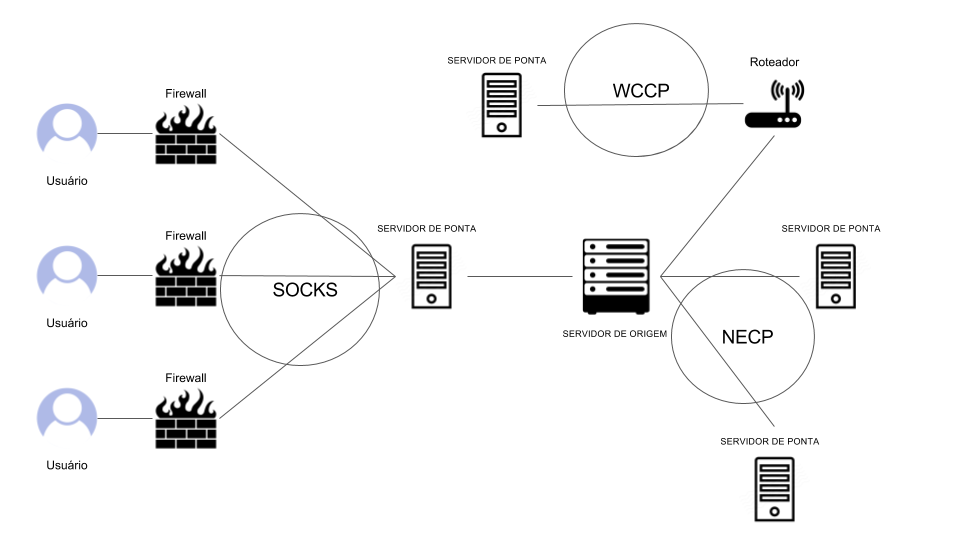
\includegraphics[width=10cm]{Figuras/protocolos_interacao_elementos.png} 
\label{figura:protocolos_interacao_elementos}
\end{figure}

\subsubsection{Intera\c{c}\~oes de cache}

\subsubsection{HTCP}
HTCP - Hypertext Caching Protocol
\begin{itemize}
\item Protocolo para descobri Caches HTTP;
\item Suporte ao HTTP 1.0;
\item Permite incluir cabeçalhos nas respostas;
\item Podem ser enviados via TCP/UDP;
\item Devem ser resilientes \`a falhas.
\end{itemize}

\subsubsection{ICP}
ICP - Internet Cache Protocol
\begin{itemize}
\item Protocolo de mensagem leve;
\item Utilizado para comunica\c{c}\~ao de Caches;
\item Utiliza consultas para determinar localiza\c{c}\~ao mais apropriada;
\item Suporte ao HTTP 0.9;
\item Comunica-se com caches vizinhos;
\item recebe MISS ou HIT como resposta;
\item Enviado via UDP;
\item Falha por timeout indica caminho quebrado;
\item Fornece informa\c{c}\~oes para balanceamento atrav\'es das medidas de perda.
\end{itemize}

\subsubsection{HTCP x ICP}
HTCP x ICP
\begin{itemize}
\item HTCP permite envio via UDP e TCP;
\item HTCP permite incluir apenas os cabeçalhos nas respostas;
\item HTCP consegue monitorar conte\'udo de caches remotos(n\~ao vizinhos)
\item ICP permite monitoramento de falhas e assim controle para balanceamento
\end{itemize}

\subsubsection{CARP}
CARP -  Cache Array Routing Protocol
Protocolo de armazenamento distribu\'ido baseado em uma lista conhecida de proxies suavemente acoplada e uma fun\c{c}\~ao hash para dividir o espa\c{c}o URL entre esses proxies.
\begin{itemize}
\item Cliente HTTP pode enviar requisi\c{c}\~ao \`a qualquer proxy da lista.
\end{itemize}

\subsubsection{Cache Digest}
Cache Digest
Protocolo de interc\^ambio e formato de dados entre caches.
\begin{itemize}
\item Fornecem um resumo dos conte\'udos na resposta;
\item Soluciona os problemas de congestionamento e timeout;
\item Torna poss\'ivel determinar se um servidor possui em cache um conte\'udo;
\item Executado via HTTP ou FTP;
\item Cont\'em tempo de expira\c{c}\~ao na resposta;
\item Podem ser utilizados para eliminar redund\^ancia.
\end{itemize}

\subsection{Sele\c{c}\~ao e entrega de conte\'udo}
\begin{itemize}
	\item Full - site
	\item Partial - site
\end{itemize}

\subsubsection{Full - site}
\begin{itemize}
	\item Entrega total de conte\'udo.
\end{itemize}

\subsubsection{Partial - site}

Tipos de distribui\c{c}\~ao:
\begin{itemize}
	\item Empirico
	\item Popularidade
\end{itemize}
Tipos de aglomera\c{c}\~oes:
\begin{itemize}
	\item Objeto
	\item Conjunto de objetos
\end{itemize}

\begin{figure}[h]
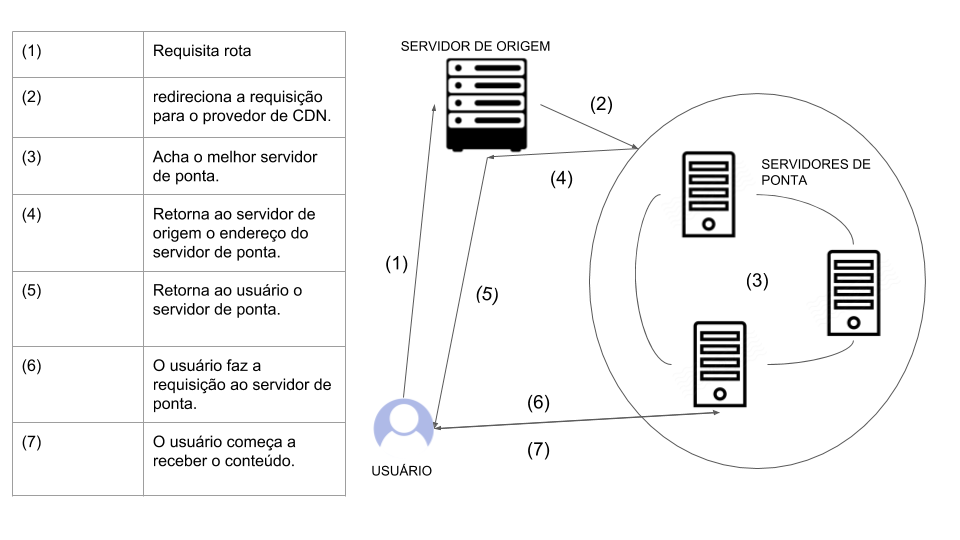
\includegraphics[width=10cm]{Figuras/entrega_conteudo.png} 
\label{figura:entrega_conteudo}
\end{figure}

\subsubsection{Exemplo}

\begin{figure}[h]
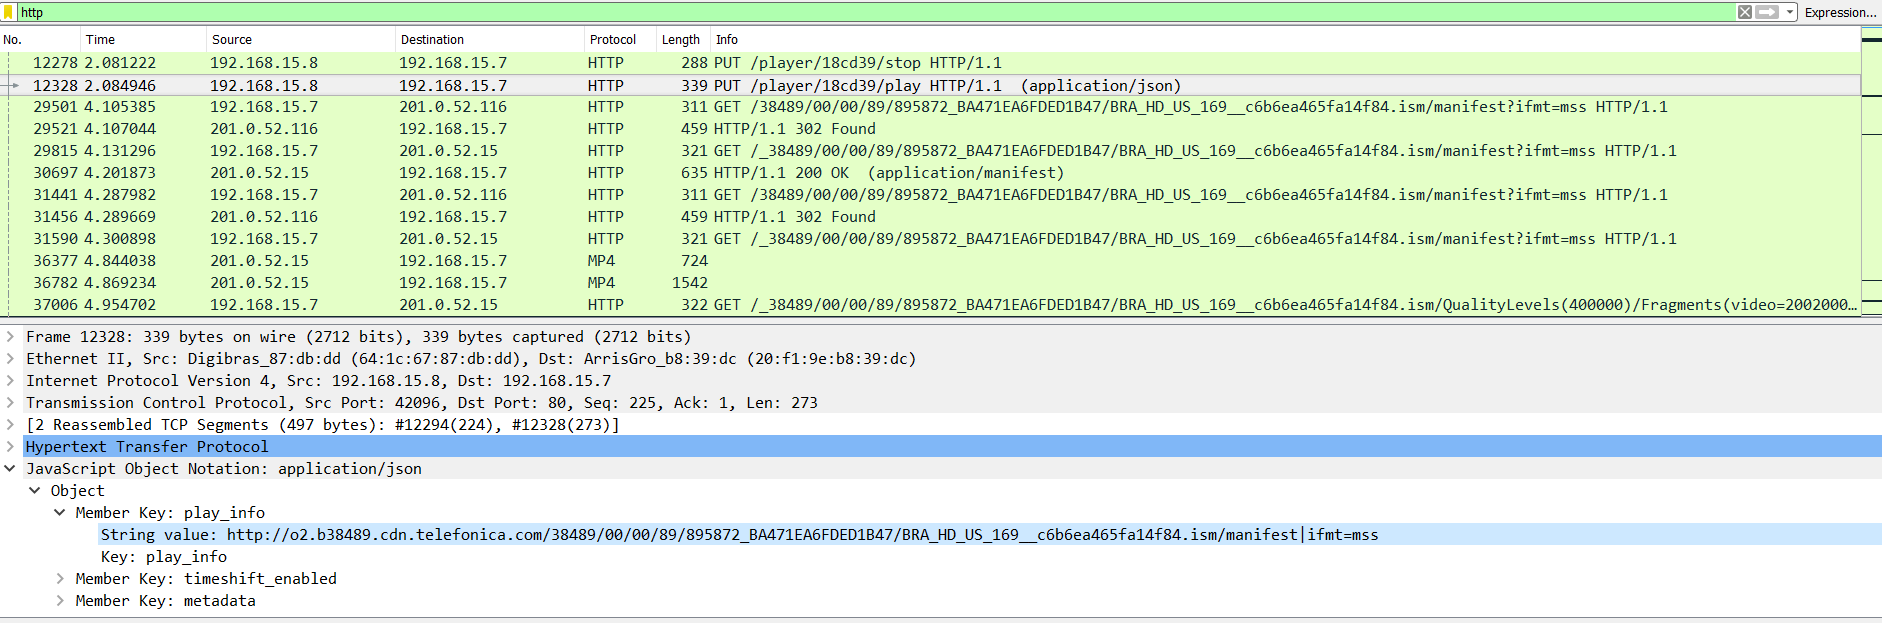
\includegraphics[width=10cm]{Figuras/exemplo_vod_1.png} 
\label{figura:exemplo_vod_1}
\end{figure}

\begin{figure}[h] 
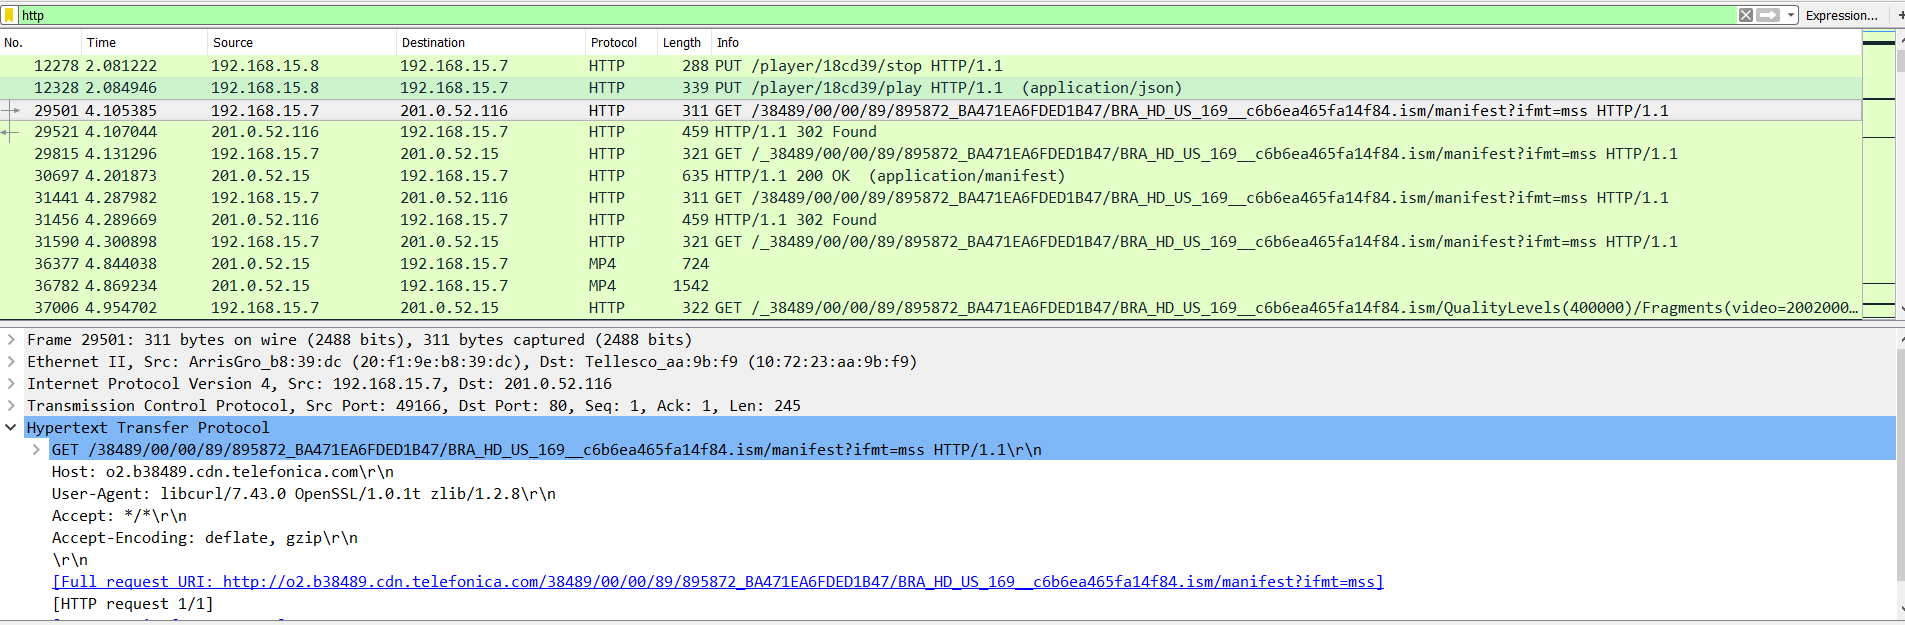
\includegraphics[width=10cm]{Figuras/exemplo_vod_2.png} 
\label{figura:exemplo_vod_2}
\end{figure}

\begin{figure}[h] 
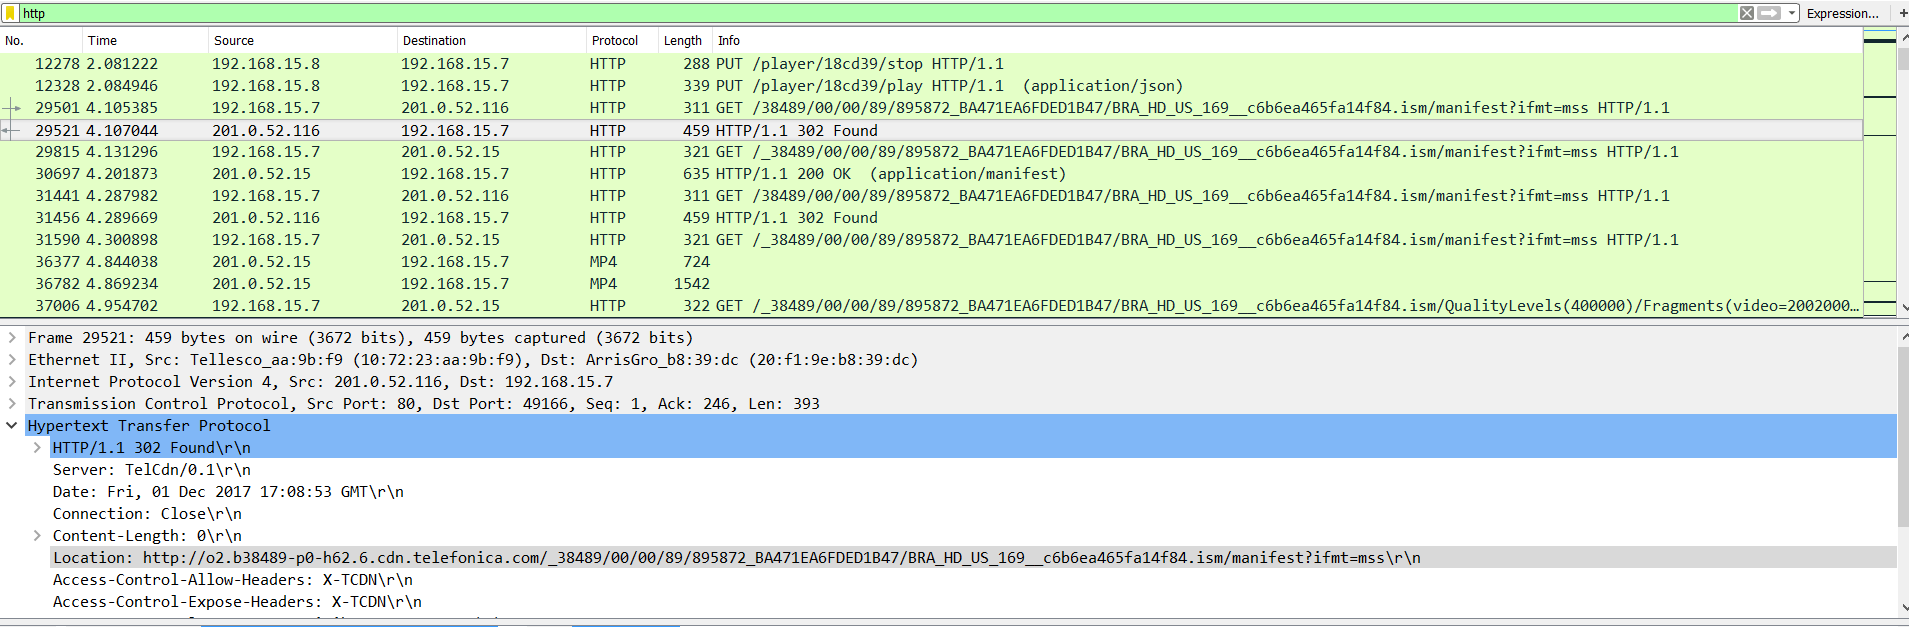
\includegraphics[width=10cm]{Figuras/exemplo_vod_3.png} 
\label{figura:exemplo_vod_3}
\end{figure}

\begin{figure}[h]
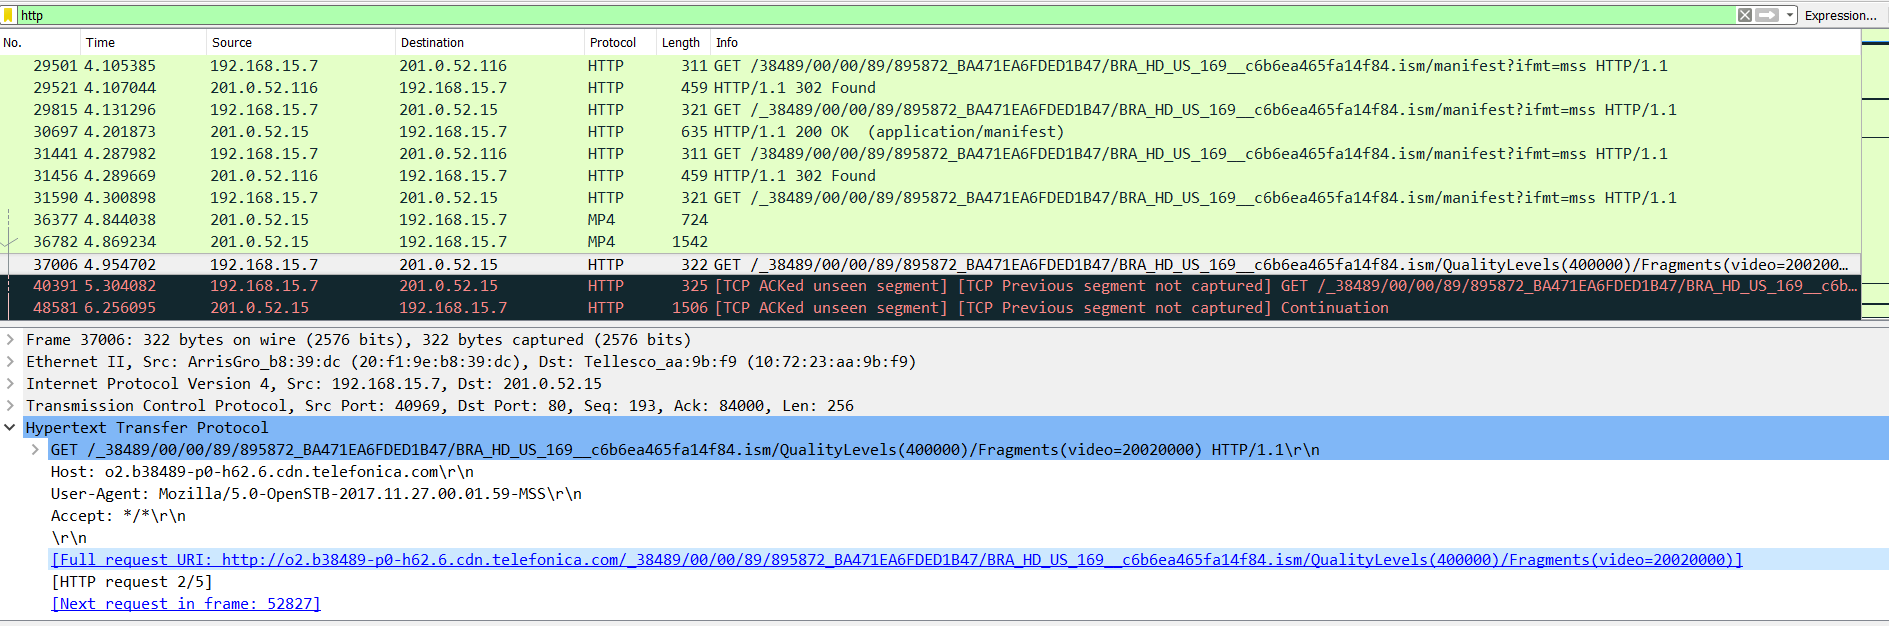
\includegraphics[width=10cm]{Figuras/exemplo_vod_4.png} 
\label{figura:exemplo_vod_4}
\end{figure}